\chapter{Finanzen}
\label{chap:finanzen}

\section{Verkaufspreis Analyse}
Um eine Idee davon zu erhalten, welchen Marktwert eine Smoilet 2.0 hat, haben wir hierf\"ur folgende Indikatoren untersucht.

\begin{itemize}
\item Wieviel kostet ein Gadget durchschnittlich
\item Was ist ein Tech User bereit f\"ur eine Smoilet 2.0 zu bezahlen 
\item Wie viele Schweizer w\"urden eine Smoilet 2.0 kaufen und was w\"urden diese daf\"ur bezahlen
\item Wer ist \"uberhaupt unsere Zielgruppe 
\end{itemize}

Bei einer Befragung von Tech Users wurden s\"amtliche Studenten der Berner Fachhochschule und Fachhochschule Nordwestschweiz der Fachrichtung Informatik, Medizininformatik, Wirtschaft Informatik, Elektrotechnik befragt, wie viel Sie f\"ur eine Smoilet 2.0 zahlen w\"urden. Von den Insgesamt 2456 Studenten antworteten 402, und es ergab sich einen Durchschnittspreis von \textbf{Fr. 46.52}. \\
Von den 402 Studenten die Antworteten waren 329 (13.4\% des Totals) Studenten am Kauf einer Smoilet 2.0 interessiert.\\
Bei einer weiteren Befragung der Schweizer Bev\"olkerung wurden 1562 Leute via Telefon und auf der Strasse (Raum Bahnhof Bern, Olten und Z\"urich) befragt, ob sie eine Smoilet 2.0 kaufen w\"urden. Zus\"atzlich wurde die Leute noch nach ihrem Alter, Beruf und Geschlecht befragt.

\begin{figure}[H]
\centering
		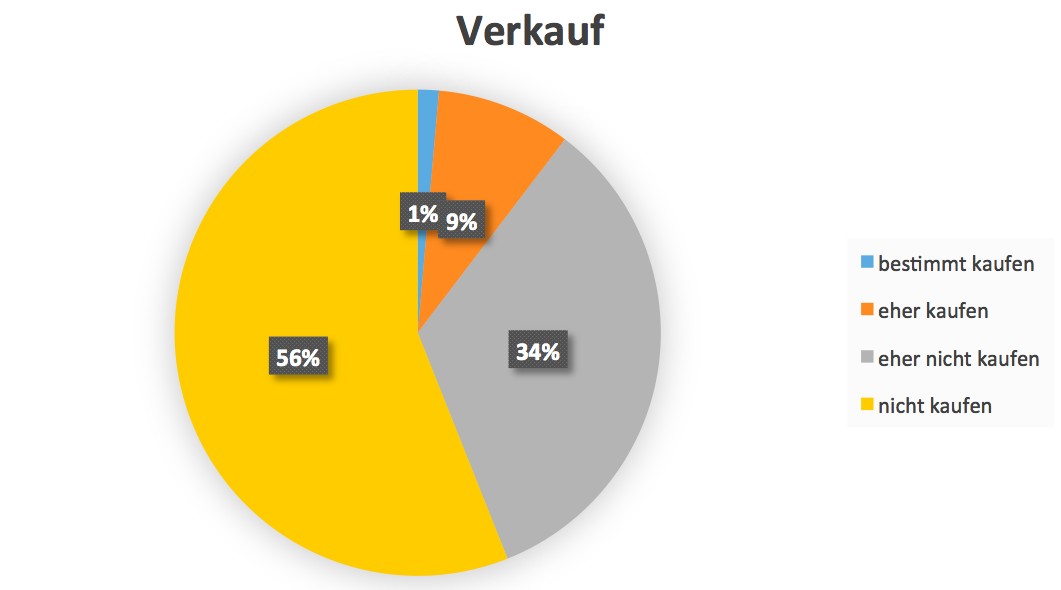
\includegraphics[scale=0.3]{bilder/marktpot.png}
\caption{Markpotential Umfrage}
\label{fig:marktpot}
\end{figure}

Hochgerechnet auf die Schweizer Bev\"olkerung ergibt sich ein Marktpotential von ca. 80000 Kunden. \\
Der ermittelte Durchschnittspreis der 1562 befragten Personen, welche eine Smoilet 2.0 kaufen oder eher kaufen w\"urden, bel\"auft sich auf \textbf{Fr. 21.95} pro Smoilet 2.0.

\subsection{Gadget Durchschnittspreise}
Hierzu haben wir 100 Artikel bei \textit{Digitec.ch}, die unter dem Suchbegriff "Gadget" gefunden wurden, analysiert und den Durchschnittspreis ermittelt. Aus folgenden Kategorien wurden Gadgets gefunden:
\begin{itemize}
\item	Activity Tracker
\item B\"uro Accessoire
\item Games
\item Gaming Figur
\item Modellbau Zubeh\"or Diverses
\item RC Gadgets (Drohnen, Modellflieger, Modell Autos etc.) 
\item Smartwatch
\item Spielsteuerung
\item Taschenlampe
\item Velobeleuchtung
\item Micro Controller (Arduino, Tinkerforge, Raspberry Pi)
\end{itemize}

Jede Kategorie wurde nach Preis sortiert, anschliessend jeweils 5 Produkte unter und \"uber dem Median ausgesucht. Somit wurden aus jeder Kategorie 10 Gadgets im Total 110 Preise Analysiert. Dies ergab einen Durchschnittspreis von \textbf{Fr. 164.38} pro Gadget. Dieser Durchschnittpreis ist natürlich relativ zu den analysierten Produkte - Drohnen und Computer waren auch in der Liste. 

\subsection{Preisgestaltung}
Eine Befragung der Schweizer Bev\"olkerung ergab, dass von den 16 Leuten die eine Smoliet 2.0 kaufen w\"urden, diese im Schnitt 28 Jahre alt, m\"annlich und in einem Technischen Beruf t\"atig sind.
In Anbetracht der Kaufkr\"aftigen Zielgruppe und den ermittelten Durchschnittspreise ergab sich folgender Richtpreis: \textbf{Fr. 34.25}. \\
Im Wissen, dass \textit{Early Adopters} und \textit{Tech Users} bereit sind mehr f\"ur die Smoilet 2.0 zu bezahlen setzten wir den Einf\"uhrungspreis auf \textbf{Fr. 39.90}.




\section{Finanzierungskonzept}
Unser Unternehmen wird mit diesem Projekt gegr\"undet. Durch Crowdfunding kann man auf einfache Weise erfahren, ob ein Produkt f\"ur potentielle Kunden attraktiv ist oder nicht. Die Finanzierung des Projekts wird in diesem Fall durch Darlehen anstatt Eigenkapital gegr\"undet. Bei den meisten Crowdfundingplatformen muss man einen Kapitalbedarf angeben (auch Goal genannt), der die Realisierung des Projekts erm\"oglicht. Wenn der Kapitalbedarf innerhalb von 30 Tagen erreicht wird, kann das Unternehmen dieses Geld fordern und die Produktion des Produkts beginnen. Innerhalb von drei Jahren sollten dann alle Produkte geliefert werden. Das Unternehmen braucht momentan keine Werbung, weil die Kunden durch Crowdfunding gesucht werden.\\
Da das Unternehmen noch nicht existiert, mussten wir einige Werte absch\"atzen:\\
\begin{itemize}
\item \textbf{Anzahl Kunden:} Wir haben die Anzahl Kunden an der durchschnittlichen Anzahl Kunden von anderer \"ahnlichen Projekten abgesch\"atzt. Einige Projekte im IT Bereich erhalten bis zu 16000 Kunden (oder Backers). 
\item \textbf{Gewinn:} Wir m\"ochten einen Gewinn von 10000 Franken pro Jahr erreichen.
\item \textbf{Material und Produktion:} Wir haben die Materialkosten pro St\"uck bei Fr. 10.- gesch\"atzt, und die Produktionskosten (Strom, Verpackung, usw.) bei Fr. 2.- .
\end{itemize}

Erkl\"arung der \"ubrigen Kosten:\\
\begin{itemize}
\item \textbf{L\"ohne:} Unser Team besteht aus 6 Personen. \\
\begin{table}[H]
\centering
\caption{L\"ohne}
\label{L\"ohne}
\begin{tabular}{lll}
\textbf{Position} & \textbf{Monatsgehalt}  \\ \hline
  \textbf{CEO} &  Fr. 4700.- \\ \hline
 \textbf{CFO} &  Fr. 4700.- \\ \hline
 \textbf{Technischer Direktor}& Fr. 4700.-  \\ \hline
 \textbf{Mitarbeiter} &Fr.  3500.- \\ \hline
 \textbf{Durchschnitt} & Fr. 4000.-\\ \hline
\end{tabular}
\end{table}
\item \textbf{Webserver:} Um unser Produkt zu vermarkten und den Kontakt zu unseren Kunden zu pflegen.

\item \textbf{Crowdfunding Taxe:} Webseiten wie Kickstarter und Indiegogo verlangen einen Anteil von 10\% des Goals, wenn das Goal erreicht wird.
\item \textbf{Mietzins:} Fr. 700.- pro Monat
\item \textbf{Copyright:} Fr. 100.-
\item \textbf{Abschreibungen:} wir buchen Abschreibungen auf Produktionsmaschinen und sonstigem (Ankauf Fr. 5000.-), in der h\"ohe von 10\% pro Jahr (angenommene Lebensdauer: 10 Jahre).
\item \textbf{Analyse und Marketing:} Anfangsstudien die vor dem Crowdfunding gemacht wurden.
\end{itemize}
Da alle Teammitglieder Aktion\"are des Unternehmens sind, wird der Jahresgewinn auf alle Mitglieder verteilt.
\section{Steuern}
Unser Unternehmen wird seinen Sitz in Deisswil bei M\"unchenbuchsee haben. Die Steuern f\"ur einen Gewinn von Fr. 180'000.- pro Jahr betragen Fr. 23800.- im Jahr (der Gewinn wird in einer sp\"ateren Sektion behandelt und erkl\"art).
\section{Zukunft}
Wir haben die Finanzplanung f\"ur die ersten 3 Jahre erstellt. Innerhalb dieser 3 Jahre werden wir den Backers das Produkt liefern. Falls die Nachfrage vorhanden ist, planen wir eine neue Version des Smoilet Produkts in den folgenden Jahren herzustellen. 
\section{Kosten\"ubersicht}
Die nachfolgenden Tabellen illustrieren die zu erwartenden variablen und fixen Kosten. Die Fixkosten nehmen im Verlauf der weiteren Jahre ab, da z.Bsp. die Analyse und Marketing Kosten nur im ersten Jahr anfallen.
\begin{figure}[H]
	\centering
		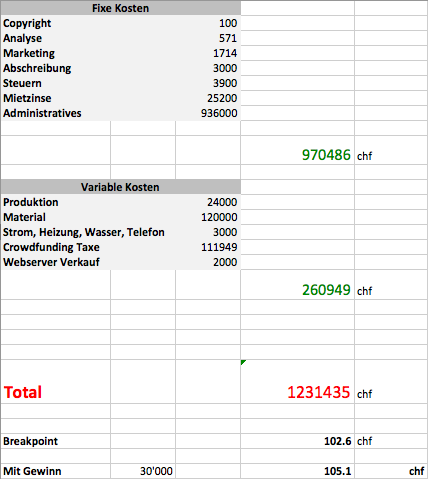
\includegraphics[scale=0.6]{bilder/3Jahre.png}
	\caption{Kosten\"ubersicht 3 Jahre}
	\label{fig:3Jahre}
\end{figure}
\begin{figure}[H]
	\centering
		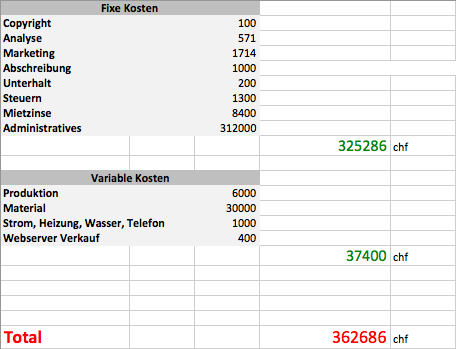
\includegraphics[scale=0.6]{bilder/Jahr1.png}
	\caption{Kosten\"ubersicht 1. Jahr}
	\label{fig:Jahr1}
\end{figure}
\begin{figure}[H]
	\centering
		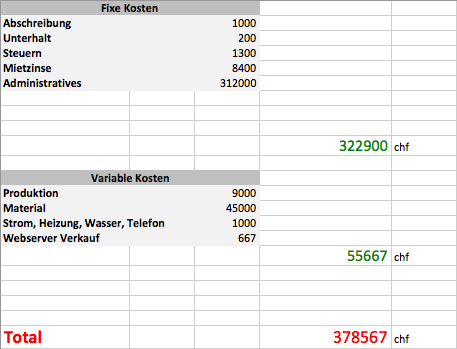
\includegraphics[scale=0.6]{bilder/Jahr2.png}
	\caption{Kosten\"ubersicht 2. Jahr}
	\label{fig:Jahr2}
\end{figure}
\begin{figure}[H]
	\centering
		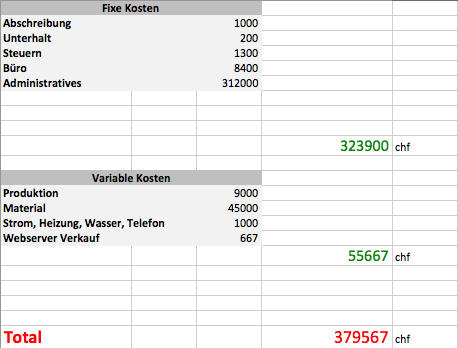
\includegraphics[scale=0.6]{bilder/Jahr3.png}
	\caption{Kosten\"ubersicht 3. Jahr}
	\label{fig:Jahr3}
\end{figure}
\begin{figure}[H]
	\centering
		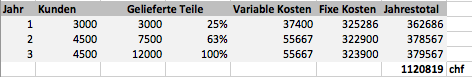
\includegraphics[scale=0.6]{bilder/kosten_ubersicht.png}
	\caption{Jahrestotal}
	\label{fig:Jahrestotal}
\end{figure}
\section{Kapitalbedarf}
Der berechnete Preis pro St\"uck is mit dem Lohn von 6 Ingenieure viel zu hoch um guten Markterfolg zu haben. Darum haben wir uns entschieden, unsere L\"ohne auszuschliessen und ehramtlich zu arbeiten. Der Gewinn kann dann noch bis zu 185'000 Fr. maximiert werden, um einen Preis von 39.90 Fr. pro St\"uck zu erhalten.
\begin{figure}[H]
	\centering
		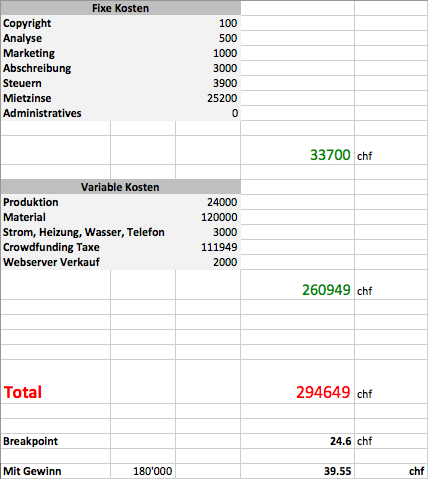
\includegraphics[scale=0.6]{bilder/ehramtlich.png}
	\caption{Kosten\"ubersicht ohne Ingenieurl\"ohne}
	\label{fig:ehramtlich}
\end{figure}

\section{Fazit}
Um den Finanzteil mit einer realistischen Planerfolgsrechnung abzuschliessen, w\"aren wir auf genaue Angaben \"uber Kosten angewiesen. Leider ist es im Rahmen dieser Arbeit nahezu unm\"oglich, an diese Zahlen zu gelangen. Ziel des Crowdfundings liegt nicht prim\"ar in der Umsatzsteigerung, sondern in der Gewinnmaximierung durch Kostenersparnisse in Bezug auf Werbung und Kundensuche. 